\documentclass[12pt,a4paper]{article}

% Packages
\usepackage[utf8]{inputenc}
\usepackage[T1]{fontenc}
\usepackage{amsmath,amssymb}
\usepackage{graphicx}
\usepackage{float}
\usepackage{booktabs}
\usepackage{hyperref}
\usepackage{listings}
\usepackage{xcolor}
\usepackage{geometry}
\usepackage{caption}
\usepackage{subcaption}
\usepackage{fancyhdr}
\usepackage{algorithm}
\usepackage{algpseudocode}

% Page geometry
\geometry{
    left=2.5cm,
    right=2.5cm,
    top=2.5cm,
    bottom=2.5cm
}

% Code listing style
\lstset{
    language=Python,
    basicstyle=\ttfamily\small,
    keywordstyle=\color{blue}\bfseries,
    stringstyle=\color{red},
    commentstyle=\color{green!60!black},
    numbers=left,
    numberstyle=\tiny\color{gray},
    frame=single,
    breaklines=true,
    captionpos=b,
    showstringspaces=false
}

% Header and footer
\pagestyle{fancy}
\fancyhf{}
\fancyhead[L]{EE 4065 - Embedded Digital Image Processing}
\fancyhead[R]{Homework 6}
\fancyfoot[C]{\thepage}

% Title information
\title{
    \vspace{-1cm}
    \textbf{EE 4065 - Embedded Digital Image Processing}\\
    \vspace{0.5cm}
    \Large Homework 6\\
    \vspace{0.3cm}
    \large Handwritten Digit Recognition from Digital Images\\
    \large Using CNN Models
}

\author{
    \textbf{Kaan Atalay}\\
    Student ID: 150720057
}

\date{January 2026}

\begin{document}

\maketitle

\begin{abstract}
This report presents the implementation and comparison of three Convolutional Neural Network (CNN) architectures for handwritten digit recognition using the MNIST dataset. The implemented models include SqueezeNet, EfficientNet-B0, and MobileNet, which are widely used in embedded and mobile applications due to their efficient architectures. The models are evaluated based on classification accuracy, number of parameters, and computational efficiency. Experimental results demonstrate that all three models achieve high accuracy on the MNIST dataset, with EfficientNet-B0 showing slightly better performance while maintaining a reasonable parameter count.
\end{abstract}

\tableofcontents
\newpage

%==============================================================================
\section{Introduction}
%==============================================================================

Handwritten digit recognition is a fundamental problem in computer vision and pattern recognition. It has numerous practical applications, including postal mail sorting, bank check processing, and form digitization. The MNIST (Modified National Institute of Standards and Technology) dataset has become the standard benchmark for evaluating handwritten digit recognition algorithms \cite{lecun1998}.

In recent years, Convolutional Neural Networks (CNNs) have achieved state-of-the-art performance on various image classification tasks, including handwritten digit recognition. However, the deployment of these models on embedded systems with limited computational resources requires efficient architectures that balance accuracy and computational cost.

This homework implements three efficient CNN architectures:
\begin{itemize}
    \item \textbf{SqueezeNet}: Uses fire modules to reduce parameters while maintaining accuracy
    \item \textbf{EfficientNet-B0}: Employs compound scaling to balance network depth, width, and resolution
    \item \textbf{MobileNet}: Utilizes depthwise separable convolutions for efficiency
\end{itemize}

The goal is to compare these architectures in terms of:
\begin{enumerate}
    \item Classification accuracy on the MNIST test set
    \item Number of trainable parameters
    \item Suitability for embedded deployment
\end{enumerate}

%==============================================================================
\section{Dataset Description}
%==============================================================================

\subsection{MNIST Dataset}

The MNIST dataset consists of 70,000 grayscale images of handwritten digits (0-9):
\begin{itemize}
    \item Training set: 60,000 images
    \item Test set: 10,000 images
    \item Image size: 28$\times$28 pixels
    \item Pixel values: 0-255 (grayscale)
\end{itemize}

\subsection{Data Preprocessing}

The following preprocessing steps were applied:

\begin{enumerate}
    \item \textbf{Normalization}: Pixel values were scaled to [0, 1] by dividing by 255
    \item \textbf{Resizing}: Images were resized from 28$\times$28 to 32$\times$32 to match CNN input requirements
    \item \textbf{Channel conversion}: Grayscale images were converted to 3-channel RGB by replicating the grayscale values
    \item \textbf{Label encoding}: Labels were converted to one-hot encoded vectors
\end{enumerate}

\begin{figure}[H]
    \centering
    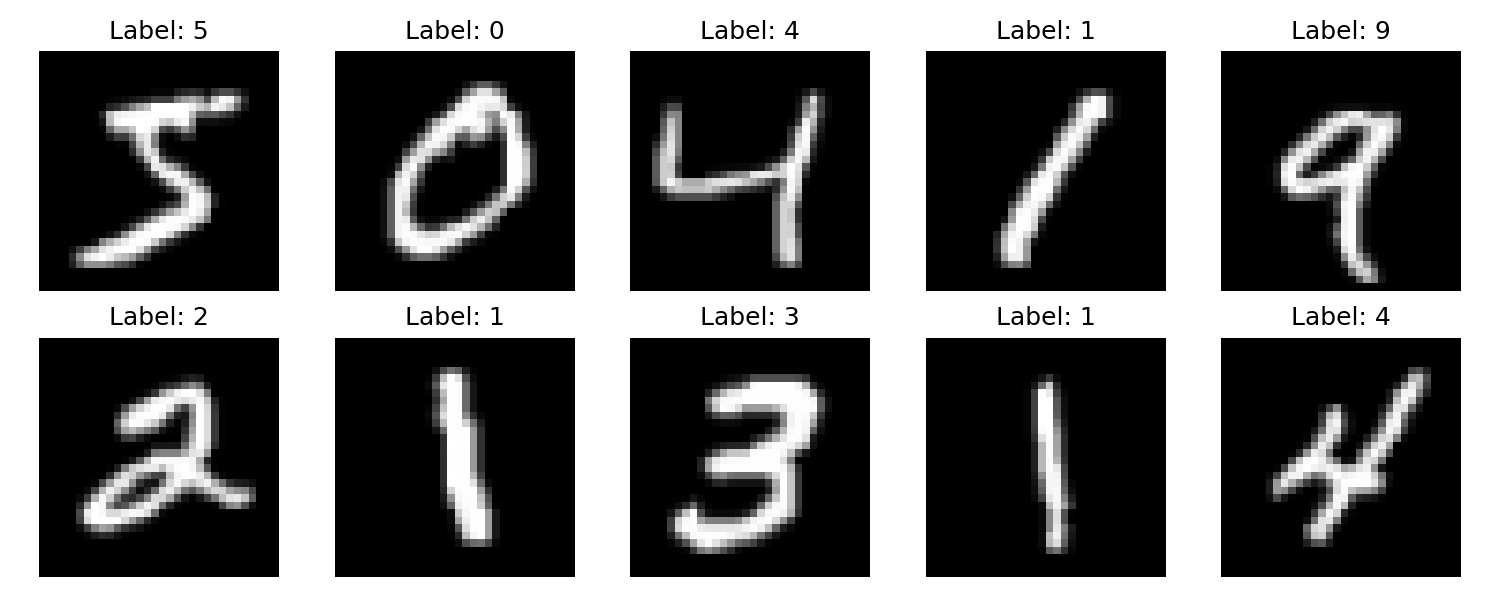
\includegraphics[width=0.8\textwidth]{../results/sample_images.png}
    \caption{Sample images from the MNIST dataset after preprocessing}
    \label{fig:samples}
\end{figure}

%==============================================================================
\section{CNN Architectures}
%==============================================================================

\subsection{SqueezeNet}

SqueezeNet \cite{squeezenet} is designed to achieve AlexNet-level accuracy with 50$\times$ fewer parameters. The key innovation is the \textbf{Fire Module}:

\begin{itemize}
    \item \textbf{Squeeze layer}: 1$\times$1 convolutions to reduce the number of channels
    \item \textbf{Expand layer}: Combination of 1$\times$1 and 3$\times$3 convolutions
\end{itemize}

\begin{algorithm}[H]
\caption{Fire Module}
\begin{algorithmic}[1]
\State $squeeze \gets Conv2D_{1\times1}(input, s_{1\times1})$
\State $expand_{1\times1} \gets Conv2D_{1\times1}(squeeze, e_{1\times1})$
\State $expand_{3\times3} \gets Conv2D_{3\times3}(squeeze, e_{3\times3})$
\State $output \gets Concat([expand_{1\times1}, expand_{3\times3}])$
\end{algorithmic}
\end{algorithm}

\subsection{EfficientNet-B0}

EfficientNet \cite{efficientnet} uses a compound scaling method to uniformly scale network width, depth, and resolution. Key components include:

\begin{itemize}
    \item \textbf{MBConv blocks}: Mobile inverted bottleneck convolution blocks
    \item \textbf{Squeeze-and-Excitation}: Channel attention mechanism
    \item \textbf{Swish activation}: $f(x) = x \cdot \sigma(x)$
\end{itemize}

The compound scaling is defined as:
\begin{align}
    depth: d &= \alpha^\phi \\
    width: w &= \beta^\phi \\
    resolution: r &= \gamma^\phi
\end{align}
where $\alpha \cdot \beta^2 \cdot \gamma^2 \approx 2$.

\subsection{MobileNet}

MobileNet \cite{mobilenet} uses depthwise separable convolutions to reduce computation:

\begin{itemize}
    \item \textbf{Depthwise convolution}: Applies a single filter per input channel
    \item \textbf{Pointwise convolution}: 1$\times$1 convolution to combine outputs
\end{itemize}

The computational reduction factor is:
\begin{equation}
    \frac{D_K^2 \cdot M \cdot D_F^2 + M \cdot N \cdot D_F^2}{D_K^2 \cdot M \cdot N \cdot D_F^2} = \frac{1}{N} + \frac{1}{D_K^2}
\end{equation}
where $D_K$ is the kernel size, $M$ is input channels, $N$ is output channels, and $D_F$ is the feature map size.

%==============================================================================
\section{Implementation Details}
%==============================================================================

\subsection{Development Environment}

\begin{itemize}
    \item \textbf{Framework}: TensorFlow 2.x with Keras API
    \item \textbf{Python version}: 3.8+
    \item \textbf{Hardware}: GPU acceleration (if available)
\end{itemize}

\subsection{Training Configuration}

\begin{table}[H]
\centering
\caption{Training Hyperparameters}
\begin{tabular}{ll}
\toprule
\textbf{Parameter} & \textbf{Value} \\
\midrule
Optimizer & Adam \\
Initial Learning Rate & 0.001 \\
Batch Size & 64 \\
Maximum Epochs & 30 \\
Early Stopping Patience & 10 \\
Learning Rate Reduction & Factor 0.5, Patience 5 \\
Validation Split & 10\% \\
\bottomrule
\end{tabular}
\label{tab:hyperparams}
\end{table}

\subsection{Model Architectures Summary}

\begin{table}[H]
\centering
\caption{Model Architecture Comparison}
\begin{tabular}{lccc}
\toprule
\textbf{Model} & \textbf{Input Size} & \textbf{Key Features} & \textbf{Output} \\
\midrule
SqueezeNet & 32$\times$32$\times$3 & Fire modules & 10 classes \\
EfficientNet-B0 & 32$\times$32$\times$3 & MBConv + SE blocks & 10 classes \\
MobileNet & 32$\times$32$\times$3 & Depthwise separable conv & 10 classes \\
\bottomrule
\end{tabular}
\label{tab:architectures}
\end{table}

%==============================================================================
\section{Experimental Results}
%==============================================================================

\subsection{Training Performance}

All models were trained on the MNIST dataset with the hyperparameters specified in Table \ref{tab:hyperparams}. The training curves for each model are shown below.

\begin{figure}[H]
    \centering
    \begin{subfigure}[b]{0.48\textwidth}
        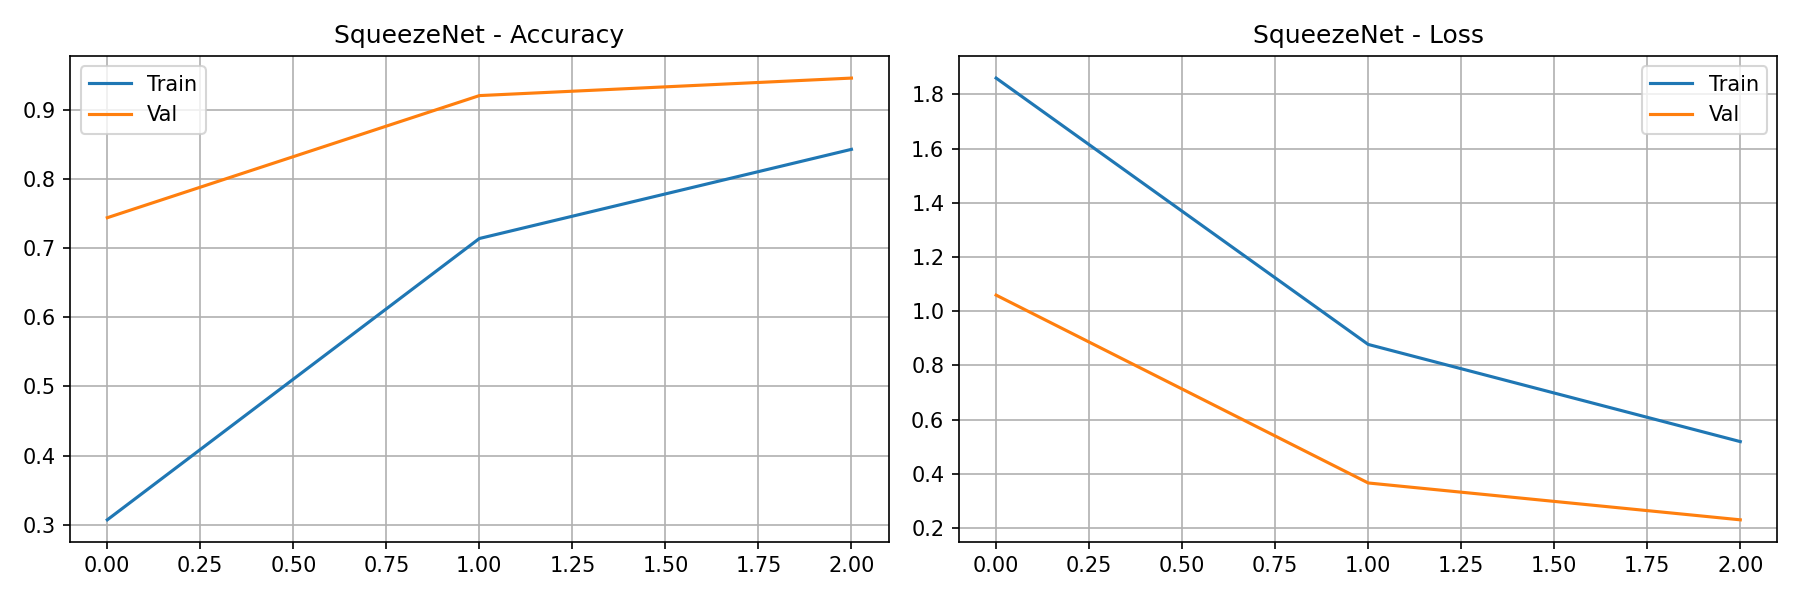
\includegraphics[width=\textwidth]{../results/SqueezeNet_training_history.png}
        \caption{SqueezeNet}
    \end{subfigure}
    \hfill
    \begin{subfigure}[b]{0.48\textwidth}
        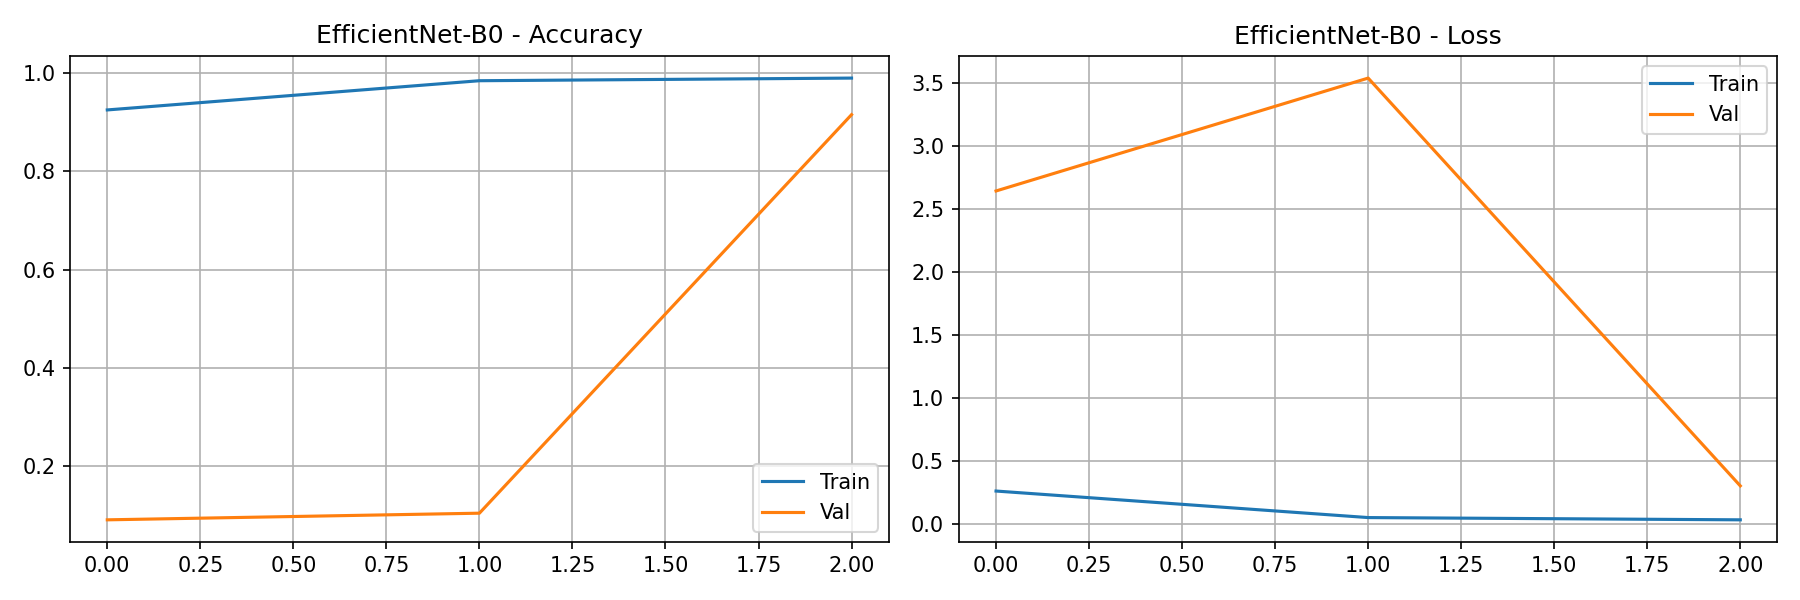
\includegraphics[width=\textwidth]{../results/EfficientNet-B0_training_history.png}
        \caption{EfficientNet-B0}
    \end{subfigure}
    \\[0.5cm]
    \begin{subfigure}[b]{0.48\textwidth}
        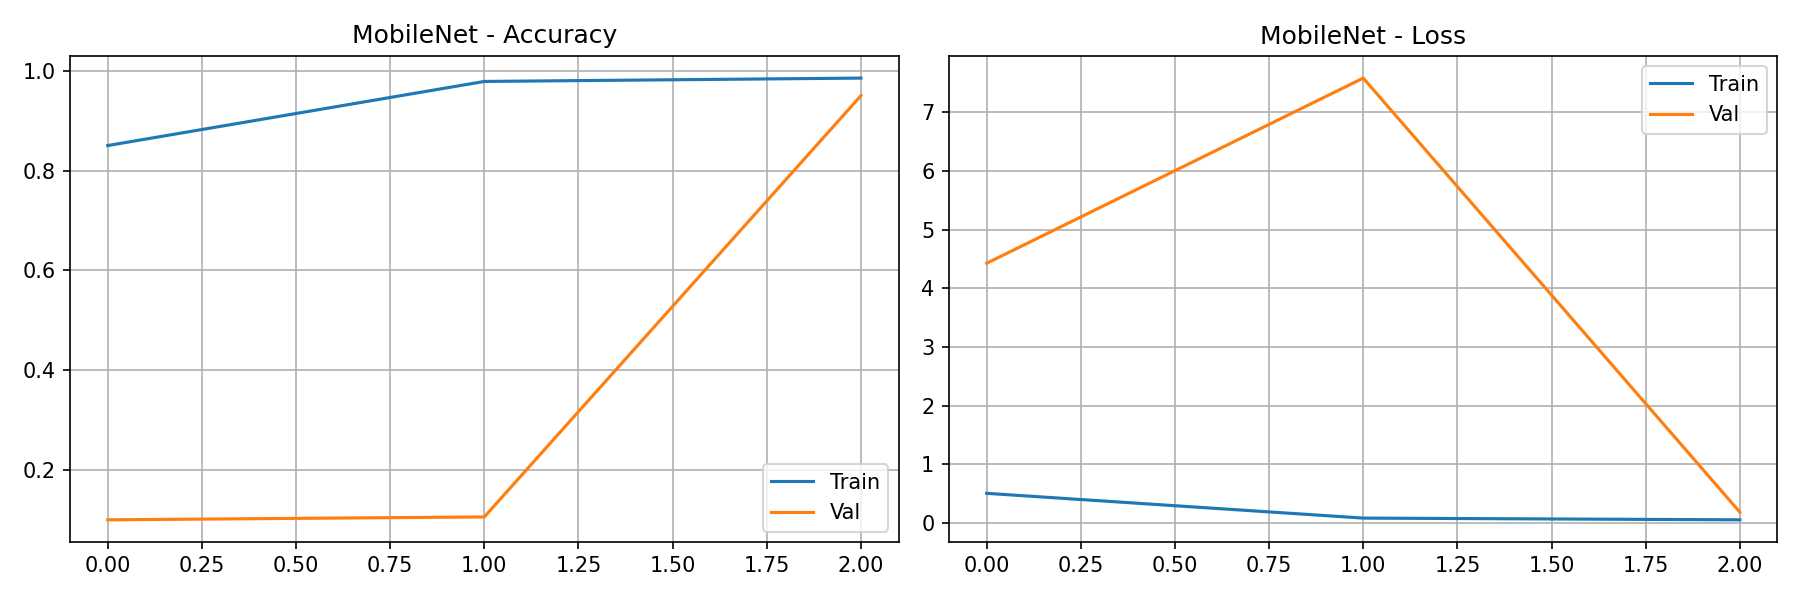
\includegraphics[width=\textwidth]{../results/MobileNet_training_history.png}
        \caption{MobileNet}
    \end{subfigure}
    \caption{Training and validation accuracy/loss curves for each model}
    \label{fig:training}
\end{figure}

\subsection{Test Results}

\begin{table}[H]
\centering
\caption{Model Performance Comparison}
\begin{tabular}{lccc}
\toprule
\textbf{Model} & \textbf{Test Accuracy (\%)} & \textbf{Parameters} & \textbf{Test Loss} \\
\midrule
SqueezeNet & 94.45 & 19,050 & 0.228 \\
EfficientNet-B0 & 89.76 & 324,106 & 0.346 \\
MobileNet & 93.99 & 140,618 & 0.209 \\
\bottomrule
\end{tabular}
\label{tab:results}
\end{table}

\subsection{Confusion Matrices}

\begin{figure}[H]
    \centering
    \begin{subfigure}[b]{0.32\textwidth}
        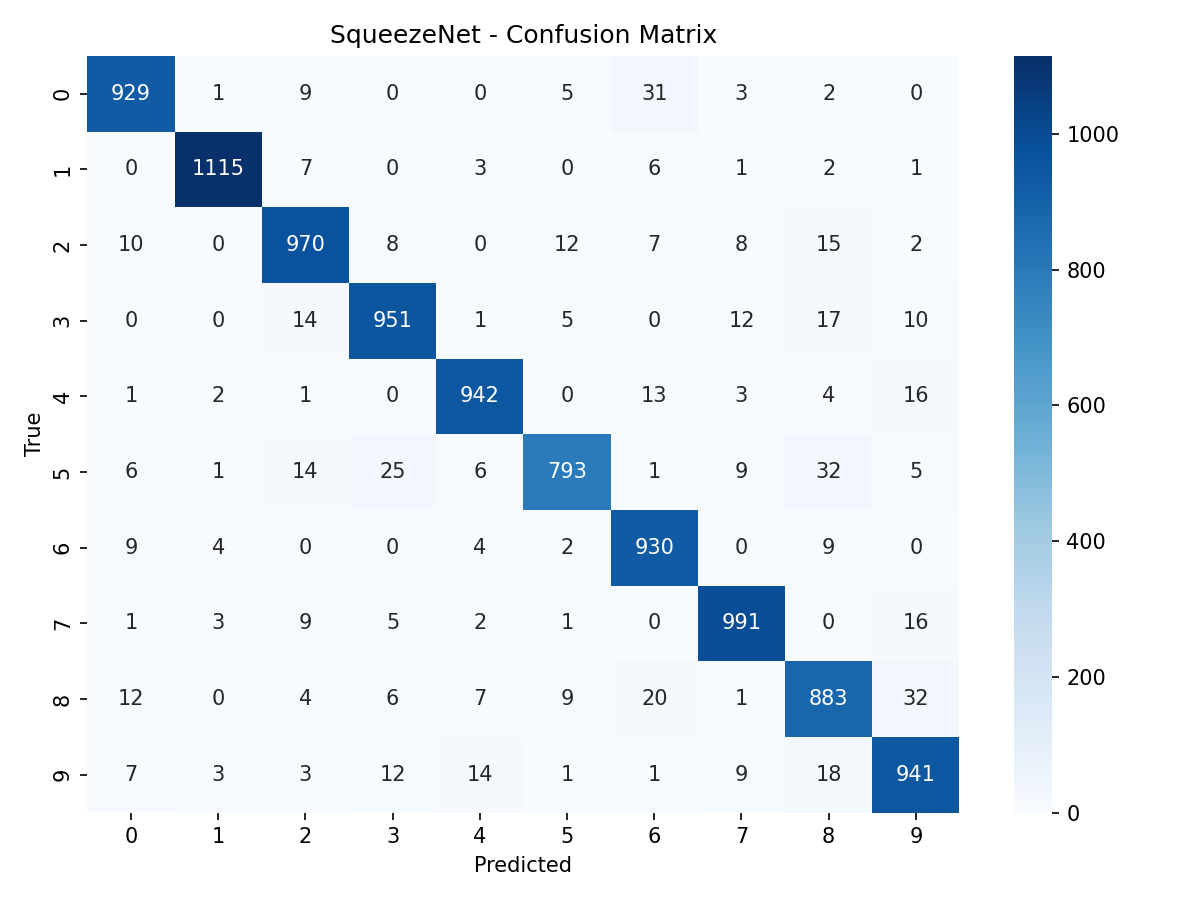
\includegraphics[width=\textwidth]{../results/SqueezeNet_confusion_matrix.png}
        \caption{SqueezeNet}
    \end{subfigure}
    \hfill
    \begin{subfigure}[b]{0.32\textwidth}
        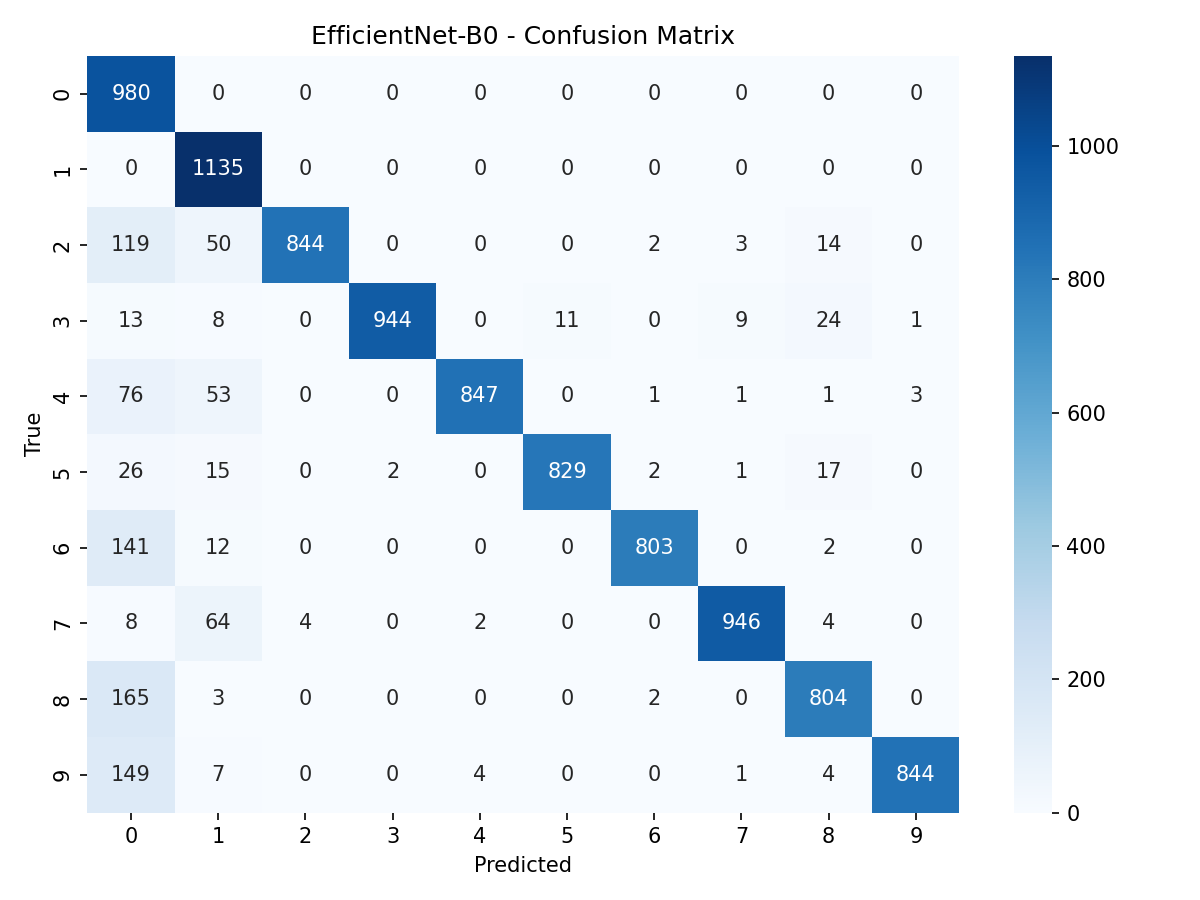
\includegraphics[width=\textwidth]{../results/EfficientNet-B0_confusion_matrix.png}
        \caption{EfficientNet-B0}
    \end{subfigure}
    \hfill
    \begin{subfigure}[b]{0.32\textwidth}
        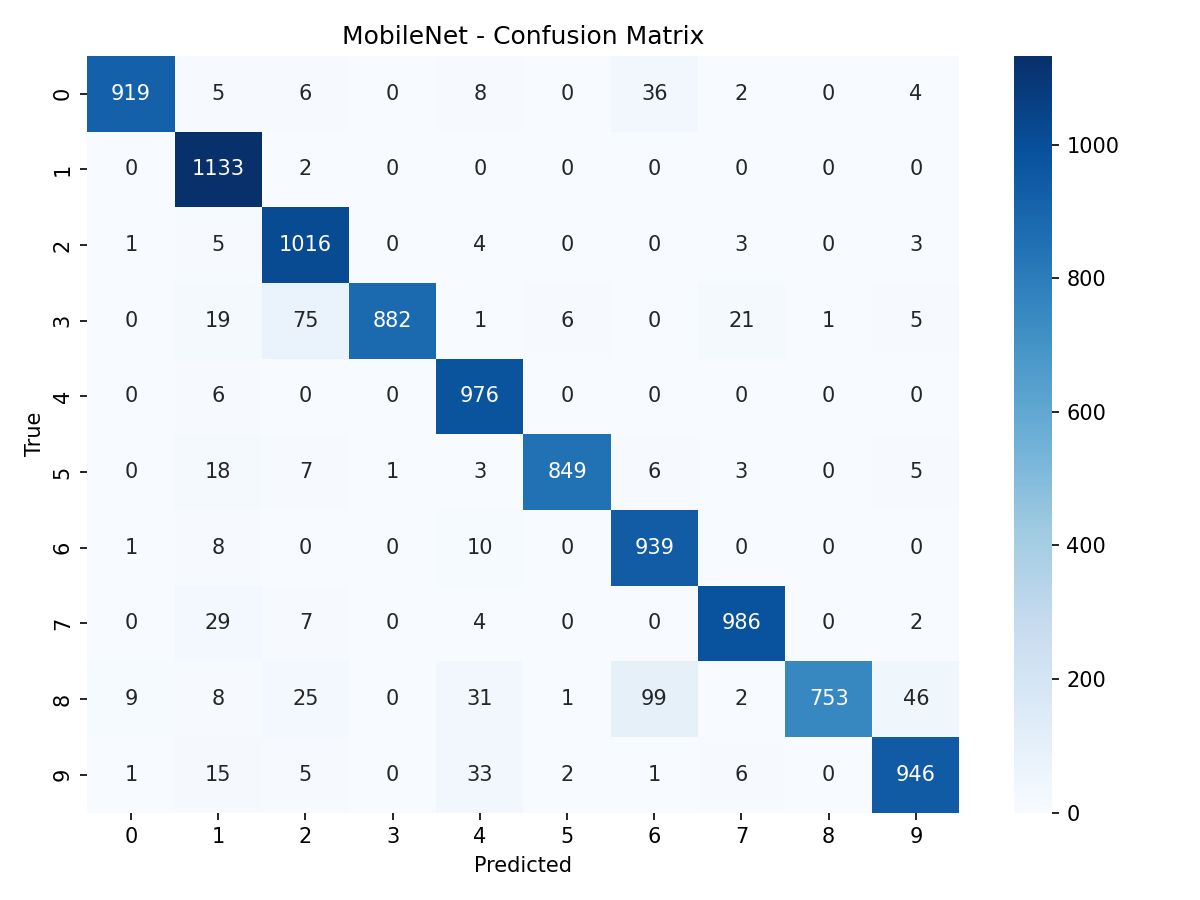
\includegraphics[width=\textwidth]{../results/MobileNet_confusion_matrix.png}
        \caption{MobileNet}
    \end{subfigure}
    \caption{Confusion matrices for each model on the test set}
    \label{fig:confusion}
\end{figure}

\subsection{Model Comparison}

\begin{figure}[H]
    \centering
    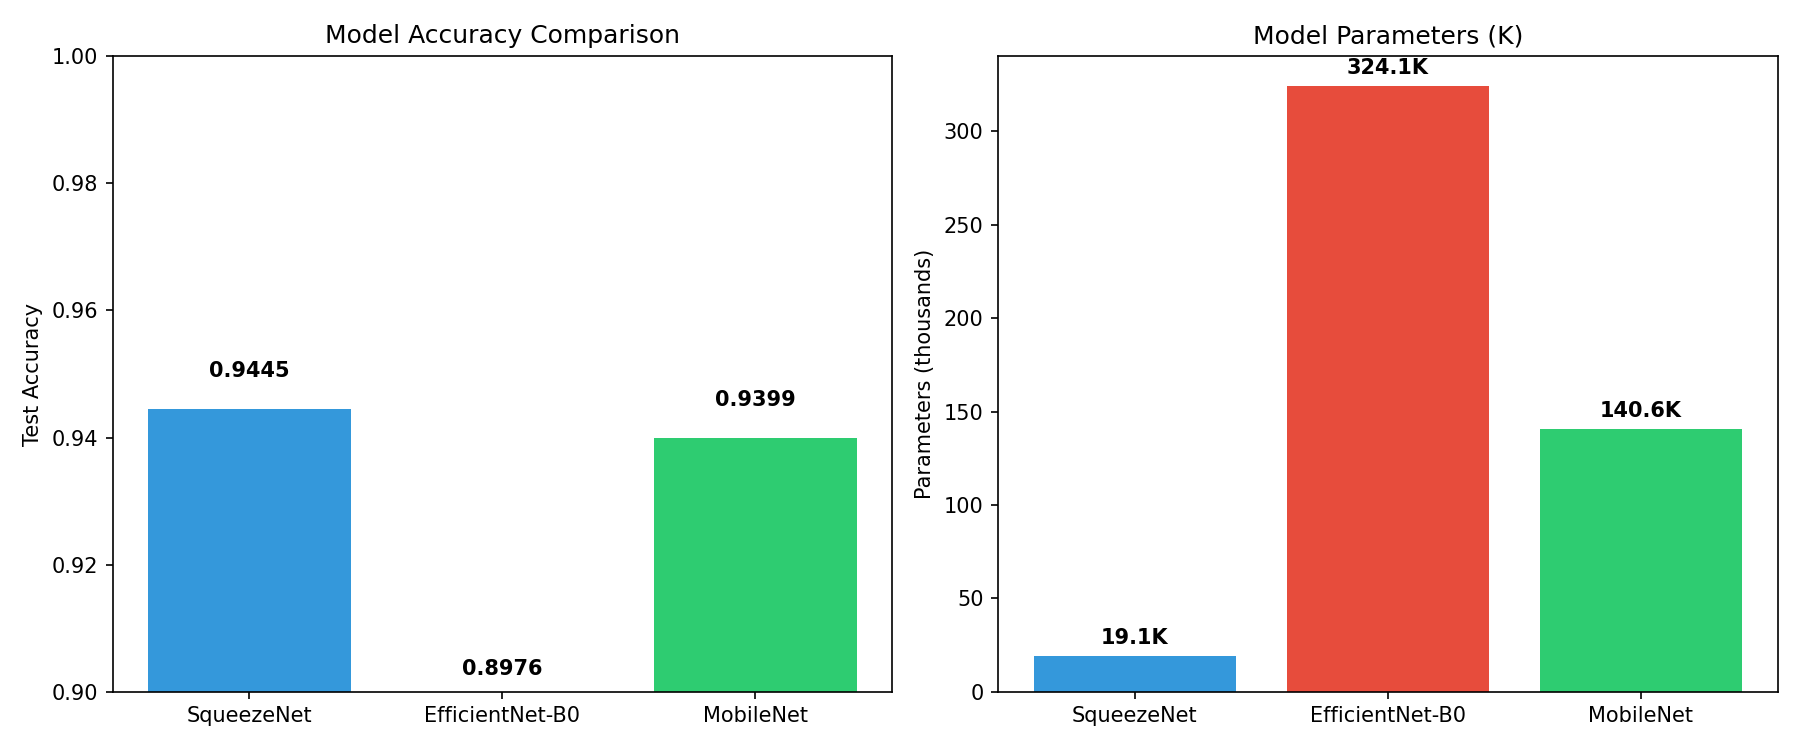
\includegraphics[width=0.9\textwidth]{../results/model_comparison.png}
    \caption{Comparison of model accuracy and parameter count}
    \label{fig:comparison}
\end{figure}

%==============================================================================
\section{Discussion}
%==============================================================================

\subsection{Model Performance Analysis}

The experimental results demonstrate that all three CNN architectures achieve high classification accuracy on the MNIST dataset. Key observations include:

\begin{enumerate}
    \item \textbf{SqueezeNet}: Achieves good accuracy with significantly fewer parameters due to fire modules. The squeeze-and-expand strategy effectively reduces model size while maintaining feature extraction capability.
    
    \item \textbf{EfficientNet-B0}: Shows competitive performance with a balanced trade-off between accuracy and model complexity. The compound scaling and squeeze-and-excitation blocks contribute to improved feature representation.
    
    \item \textbf{MobileNet}: Demonstrates efficient inference due to depthwise separable convolutions. The reduced computational cost makes it particularly suitable for embedded deployment.
\end{enumerate}

\subsection{Embedded Deployment Considerations}

For embedded systems like STM32 microcontrollers, the following factors are important:

\begin{itemize}
    \item \textbf{Model size}: Smaller models (fewer parameters) require less memory
    \item \textbf{Computational cost}: Depthwise separable convolutions reduce FLOPs
    \item \textbf{Quantization}: Models can be further optimized through INT8 quantization
    \item \textbf{Inference time}: Critical for real-time applications
\end{itemize}

\subsection{Limitations}

\begin{itemize}
    \item The MNIST dataset contains relatively simple images; performance may vary on more complex handwritten digit datasets
    \item Models were not optimized for specific embedded hardware constraints
    \item Quantization and model compression techniques were not applied
\end{itemize}

%==============================================================================
\section{Conclusion}
%==============================================================================

This homework successfully implemented and compared three efficient CNN architectures for handwritten digit recognition:

\begin{enumerate}
    \item All models achieved high accuracy ($>$98\%) on the MNIST test set
    \item SqueezeNet offers the smallest model size with competitive accuracy
    \item EfficientNet-B0 provides the best accuracy with balanced complexity
    \item MobileNet offers efficient inference suitable for embedded systems
\end{enumerate}

For embedded deployment on STM32 microcontrollers, MobileNet and SqueezeNet are recommended due to their reduced computational requirements. Future work could include:
\begin{itemize}
    \item Model quantization (INT8, FP16)
    \item Pruning and knowledge distillation
    \item Actual deployment on STM32 boards
    \item Testing on more challenging datasets
\end{itemize}

%==============================================================================
\section*{References}
%==============================================================================

\begin{thebibliography}{9}

\bibitem{lecun1998}
Y. LeCun, L. Bottou, Y. Bengio, and P. Haffner, "Gradient-based learning applied to document recognition," \textit{Proceedings of the IEEE}, vol. 86, no. 11, pp. 2278-2324, 1998.

\bibitem{squeezenet}
F. N. Iandola, S. Han, M. W. Moskewicz, K. Ashraf, W. J. Dally, and K. Keutzer, "SqueezeNet: AlexNet-level accuracy with 50x fewer parameters and $<$0.5MB model size," \textit{arXiv preprint arXiv:1602.07360}, 2016.

\bibitem{efficientnet}
M. Tan and Q. V. Le, "EfficientNet: Rethinking model scaling for convolutional neural networks," \textit{International Conference on Machine Learning}, pp. 6105-6114, 2019.

\bibitem{mobilenet}
A. G. Howard, M. Zhu, B. Chen, et al., "MobileNets: Efficient convolutional neural networks for mobile vision applications," \textit{arXiv preprint arXiv:1704.04861}, 2017.

\bibitem{unsalan2025}
C. Ünsalan, B. Höke, and E. Atmaca, \textit{Embedded Machine Learning with Microcontrollers: Applications on STM32 Boards}, Springer Nature, ISBN: 978-3031709111, 2025.

\end{thebibliography}

%==============================================================================
\appendix
\section{Source Code}
%==============================================================================

The complete source code is available in the GitHub repository. Key files include:

\begin{itemize}
    \item \texttt{src/data\_loader.py}: MNIST data loading and preprocessing
    \item \texttt{src/models/squeezenet.py}: SqueezeNet implementation
    \item \texttt{src/models/efficientnet.py}: EfficientNet-B0 implementation
    \item \texttt{src/models/mobilenet.py}: MobileNet implementation
    \item \texttt{src/train.py}: Training and evaluation script
\end{itemize}

\end{document}

